\documentclass{labo}

\usepackage{charter}
\usepackage[utf8x]{inputenc}
\usepackage[T1]{fontenc}
\usepackage{ucs}
\usepackage{amsthm} %numéroter les questions
% \usepackage[frenchb]{babel}
\usepackage{datetime}
\usepackage{xspace} % typographie IN
\usepackage{hyperref}% hyperliens
\usepackage[all]{hypcap} %lien pointe en haut des figures
\usepackage[french]{varioref} %voir x p y
\usepackage{fancyhdr}% en têtes
\usepackage[]{graphicx} %include pictures
% \usepackage{pgfplots}
\usepackage[americanresistors,siunitx]{circuitikz}
\usepackage[]{gnuplottex}
\usepackage{ifthen}
\usepackage{mathastext} % math as standfard text : units are respecting typography conventions.
\usepackage[]{subfig}
\usepackage[]{attachfile}
\usepackage{tikz}
\usetikzlibrary{babel,positioning,calc}
\usepackage{siunitx}
\usepackage{amssymb}
\usepackage{xcolor}
\usepackage{float}
\usepackage[normalem]{ulem}
\usepackage{todonotes}

\usepackage{framed}

%%%%%%%%%%%%
% Tables
%%%%%%%%%%%%
\usepackage{booktabs}
\renewcommand{\arraystretch}{1.1} % Opens up the table a tad
\usepackage{multicol}
\usepackage{multirow}

\newboolean{koriG}
\ifx\koriG\undefined
\correction{false}
\else
\correction{true}
\fi

\newcommand{\itgv}[1]{\ifthenelse{\boolean{corrige}}{{\color{blue}#1}}{}} %si corrigé vrai...
\newcommand{\ifgv}[1]{\ifthenelse{\boolean{corrige}}{}{#1}} %si corrigé vrai...

% \correction{false}
%\correction{true}

\definecolor{darkblue}{rgb}{0,0,0.5}

%% fancy header & foot
\pagestyle{fancy}
\lhead{[EOSI40] Instrumentation labs\\ Lab 2: Building a command interface for Arduino}
\rhead{v0.9.0 \\ page \thepage}
\chead{\ifthenelse{\boolean{corrige}}{Corrigé}{}}
\cfoot{}
%%

\author{GEI}


\setlength{\parindent}{0pt}


%from SO: kinky cross for wires
\tikzset{
  declare function={% in case of CVS which switches the arguments of atan2
    atan3(\a,\b)=ifthenelse(atan2(0,1)==90, atan2(\a,\b), atan2(\b,\a));},
  kinky cross radius/.initial=+.125cm,
  @kinky cross/.initial=+, kinky crosses/.is choice,
  kinky crosses/left/.style={@kinky cross=-},kinky crosses/right/.style={@kinky cross=+},
  kinky cross/.style args={(#1)--(#2)}{
    to path={
      let \p{@kc@}=($(\tikztotarget)-(\tikztostart)$),
          \n{@kc@}={atan3(\p{@kc@})+180} in
      -- ($(intersection of \tikztostart--{\tikztotarget} and #1--#2)!%
             \pgfkeysvalueof{/tikz/kinky cross radius}!(\tikztostart)$)
      arc [ radius     =\pgfkeysvalueof{/tikz/kinky cross radius},
            start angle=\n{@kc@},
            delta angle=\pgfkeysvalueof{/tikz/@kinky cross}180 ]
      -- (\tikztotarget)}}}


\begin{document}
\tptitle{}{Lab 2: Building a command interface for Arduino}

Before you start, make sure that the relevant LabView libraries for Arduino are installed.

\begin{enumerate}
  \item Launch ``VI Package Manager'' that came with your LabView installation, and install the package ``LabView Interface for Arduino''. Launching the package manager for the first time might take a while, brace yourself.
  \begin{center}
    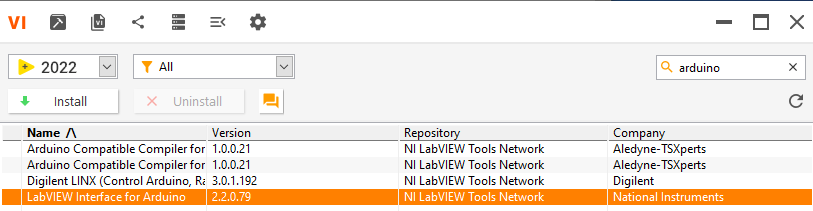
\includegraphics[width=\linewidth]{VI-package-manager.png}
  \end{center}

  \item When connecting for the first time to the Arduino board, you will need to install the LabView firmware located at: \texttt{C:\textbackslash Program Files (x86)\textbackslash National Instruments\textbackslash LabVIEW 2022\textbackslash vi.lib\textbackslash LabVIEW Interface for Arduino\textbackslash Firmware\textbackslash LIFA\_Base\textbackslash LIFA\_Base.ino}

  \item If you encounter the following error during the compilation of the firmware: \texttt{RobotIRremoteTools.cpp:5: error: 'TKD2' was not declared in this scope}, delete the library files from \texttt{C:/Program Files (x86)/Arduino/libraries/RobotIRremote}.

  \item Press the \texttt{Reset} button on the Arduino board every time you want to start a LabView program.
\end{enumerate}




\section{Interface to turn on/off the LED on pin13}
Build an interface, such as illustrated on Figure~\ref{fig:led-interface}, to control the embedded LED connected on pin 13.


\begin{figure}[ht!]
  \centering
  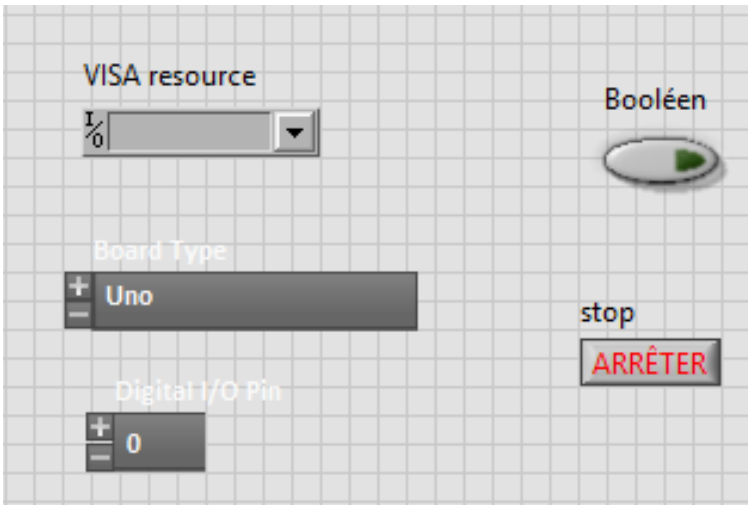
\includegraphics[width=.6\textwidth]{front-panel-LED.png}
  \caption{Front panel for controlling the LED.}
  \label{fig:led-interface}
\end{figure}

\begin{leftbar}
A few rules to follow:
\begin{enumerate}
  \item Initialize the Arduino by uploading \texttt{LIFA\_Base.ino}.
  \item Press the \texttt{Reset} button on the board.
  \item Check that the baudrates are coherent (115200 by default).
  \item Use the initialization function to start the Arduino program.
  \item Specify the appropriate \texttt{COM} port connected to your board.
  \item Finish up the program cleanly by calling the close function.
  \item If the error \texttt{5002} pops up, start the procedure over by physically disconnecting and reconnecting the board to your computer.
  \item If the Arduino does not respond, close LabView and disconnect the Arduino. Plug it back in and upload \texttt{LIFA\_Base.ino}.
  \item If the error does not go away, decrease the baudrate down to 9600.
    \begin{enumerate}
      \item In the \texttt{LIFA\_Base} software, in the \texttt{LabVIEWInterface.h} tab, where you see the keyword \texttt{DEFAULTBAUDRATE}.
      \item In your LabView program, in the initialization.

    \end{enumerate}
\end{enumerate}
\end{leftbar}




\section{Analog read}

\begin{minipage}{.4\textwidth}
Build an interface to read the analog value of the Arduino pin \texttt{A0} for which the voltage is set by a potentiometer.
Dynamically display its value in a graph and in a reservoir.
The front panel of such a system is illustrated on the right.
\end{minipage}
\hfill
\begin{minipage}{.5\textwidth}
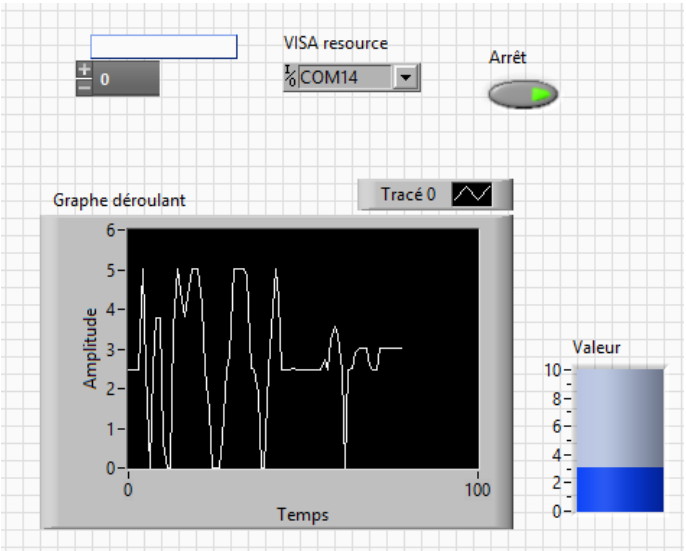
\includegraphics[width=\textwidth]{front-panel-analog.png}
\end{minipage}



\section{Controlling an RGB LED using a potentiometer}

\begin{minipage}{.45\textwidth}
Build an interface to command an RGB LED.
Each component should be controlled using a slider, as illustrated on the right.

\begin{leftbar}
Color modules:
\begin{itemize}
  \item Block diagram: Programming/Numeric/Conversion
  \item Front panel: Modern/Numeric/Vertical Pointer Slide
\end{itemize}
\end{leftbar}
\end{minipage}
\hfill
\begin{minipage}{.5\textwidth}
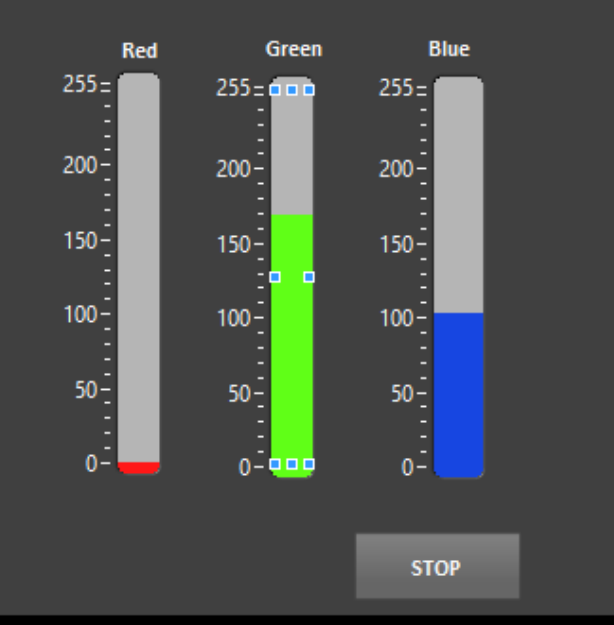
\includegraphics[width=\textwidth]{front-panel-rgb.png}
\end{minipage}



\section{X and Y axis of the joystick}\label{sec:joystick}
Build a program that reads the two analog values from the joystick and implement the necessary mathematical processing to extract its angle.


\section{Interfacing with a servomotor}
Using the VI from Section~\ref{sec:joystick}, build the command for a servomotor (see Figure~\ref{fig:servo-control}).
To fulfill this task, draw inspiration from the VI used in the Arduino library ``servo example\footnote{Located at \texttt{C:\textbackslash Program Files (x86)\textbackslash National Instruments\textbackslash LabVIEW 2022\textbackslash vi.lib\textbackslash LabVIEW Interface for Arduino\textbackslash Palette Examples}}'' (see Figure~\ref{fig:servo-block}).

\begin{figure}[ht!]
  \centering
  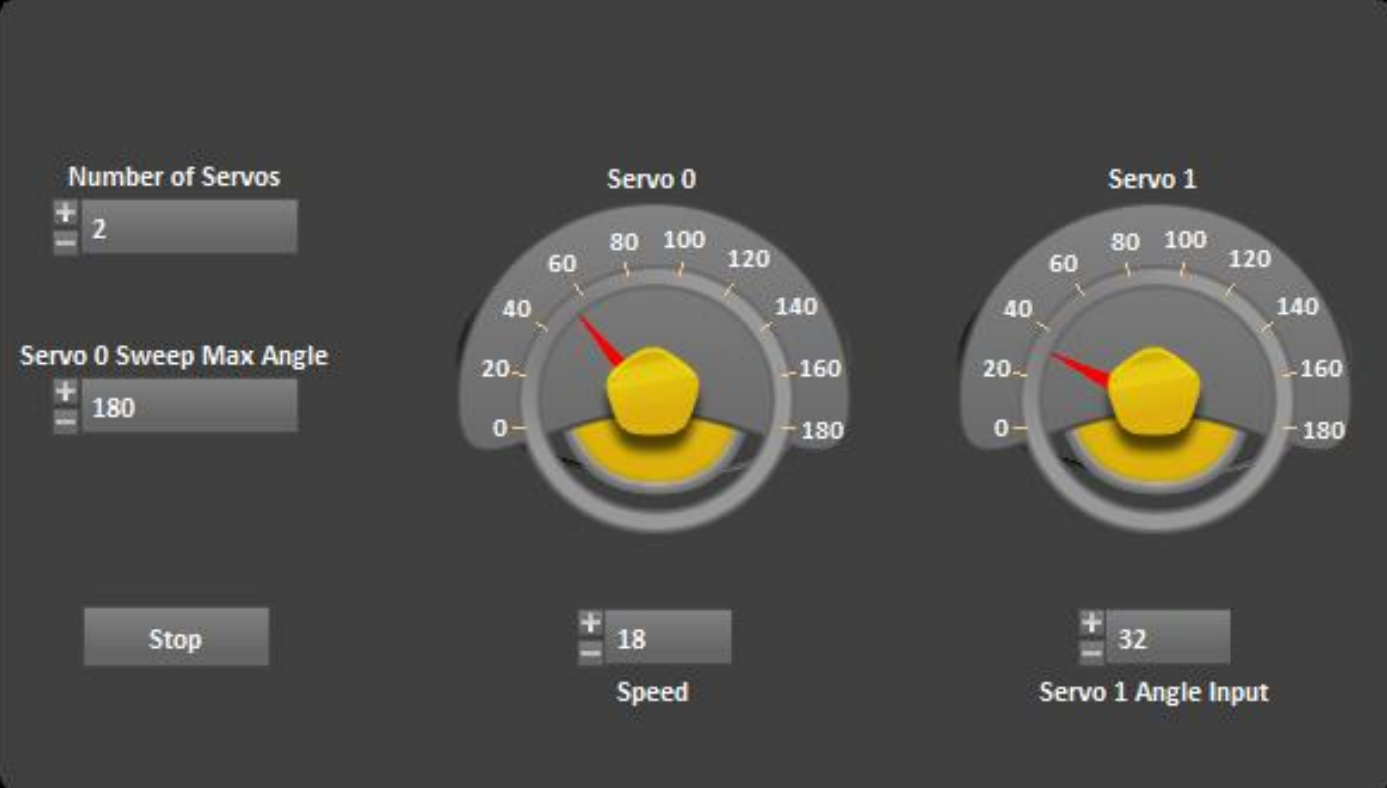
\includegraphics[width=.9\textwidth]{front-panel-servo.png}
  \caption{Front panel for controlling a servomotor.}
  \label{fig:servo-control}
\end{figure}

\begin{figure}[ht!]
  \centering
  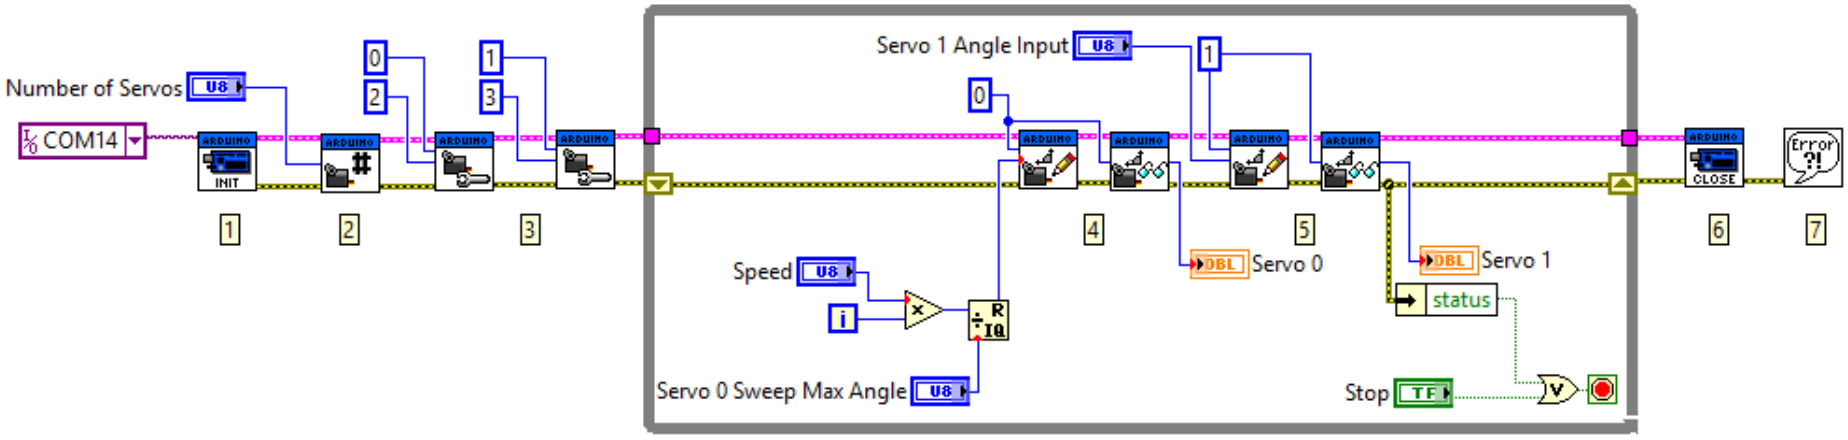
\includegraphics[width=\textwidth]{block-diagram-servo.png}
  \caption{Block diagram for controlling a servomotor.}
  \label{fig:servo-block}
\end{figure}

% \begin{figure}[ht!]
% \centering
% 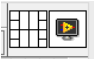
\includegraphics[]{mod-icon-conn.png}
% \caption{}\label{fig:mod-icon-conn}
% \end{figure}



% \Question{}{}
\end{document}
